\documentclass[11pt]{article}
\usepackage[margin=0.8in]{geometry}
\usepackage[T1]{fontenc}
\usepackage{lmodern,graphicx,amsmath}
\usepackage[hidelinks]{hyperref}
\begin{document}
\title{Deployed Binary-Size Cost Calculation}
\author{Research execution record}
\date{18 October 2026}
\maketitle
\noindent\textbf{Partial conditional model. No timing, attack or security claim.}

The native calculator produced 1,944 rows under the original frozen protocol,
and 2,592 under an additive amendment including zero-charge sensitivity.
Nine curve cases, four arities, six degree models, three column-work exponents
and four conversion weights occur in the amended output. Four native checks
pass, including reproduction of the historical $n=131$ anchors.

For $m=4$, $w=2$, conversion one and constant degree four, the partial-cost
gaps on the Koblitz curves of degrees 233, 283, 409 and 571 are respectively
$+15.20,+8.42,-2.30,-16.75$ bits against idealized automorphism rho.
The model includes unsuccessful attempts and relation algebra and searches
all integer subspace dimensions $4\leq\ell\leq n$.

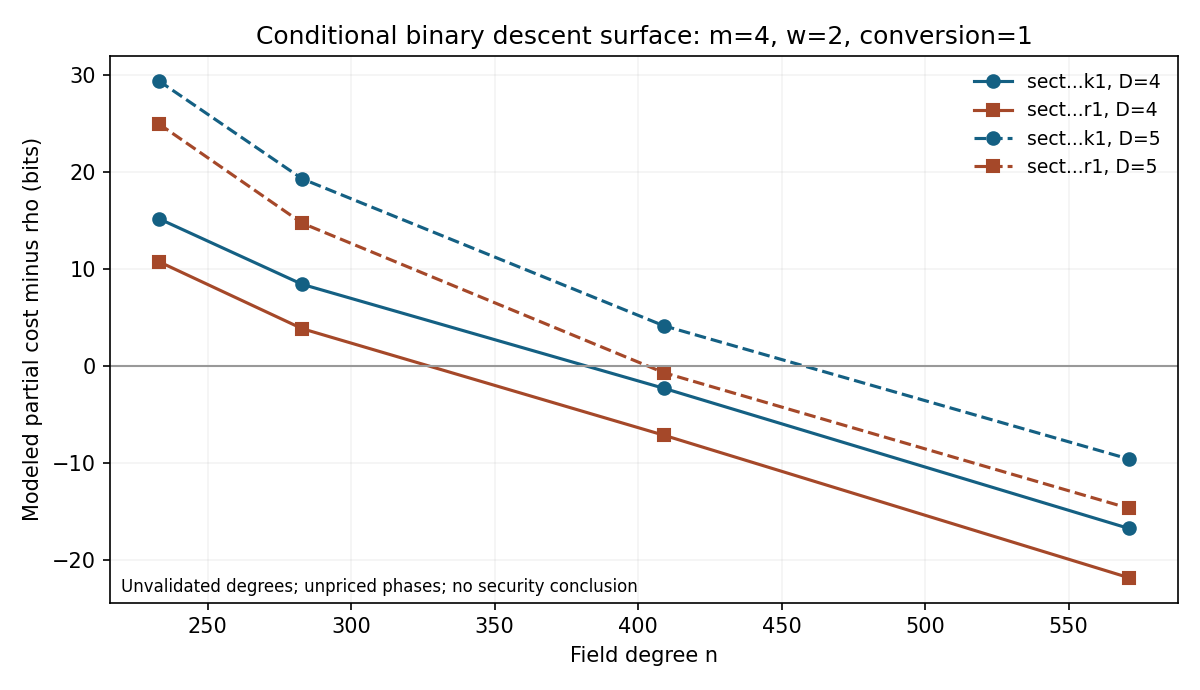
\includegraphics[width=\linewidth]{cost_surface.png}

Degree four at deployed sizes is unvalidated. Conversion from column work
to group operations is assumed, and factor-base construction, successful
extraction and other overhead are absent. Degree five changes the crossover.
Coordinate-storage estimates are not measured peak memory. Neither a modeled
negative gap nor a zero-charge arm establishes a usable attack.

\noindent\textbf{Reproduction and evidence.}
The standalone Rust crate, frozen protocol, additive amendment,
original and amended JSON, source hashes and exact commands are retained
beside this report. The original model executed at revision
\texttt{04c3c012}; the amendment at \texttt{b3a3321c}.
The initial missing-binary launch exited 127 and is recorded separately.
Python renders stored JSON only.
\end{document}
